\documentclass{beamer}
\mode<presentation>

\usepackage{array}
\usepackage{amsmath}
\usepackage[export]{adjustbox}

\usepackage{circuitikz}
\usepackage{tikz}
\usepackage{amssymb}
%\usepackage{advdate}
\usepackage{adjustbox}
\usepackage{subcaption}
\usepackage{enumitem}
\usepackage{multicol}
\usepackage{mathtools}
\usepackage{listings}
\usepackage{url}
\def\UrlBreaks{\do\/\do-}
\usetheme{Warsaw}
\usecolortheme{lily}
\setbeamertemplate{footline}
{
  \leavevmode%
  \hbox{%
  \begin{beamercolorbox}[wd=\paperwidth,ht=2.25ex,dp=1ex,right]{author in head/foot}%
    \insertframenumber{} / \inserttotalframenumber\hspace*{2ex} 
  \end{beamercolorbox}}%
  \vskip0pt%
}
\setbeamertemplate{navigation symbols}{}

\providecommand{\nCr}[2]{\,^{#1}C_{#2}} % nCr
\providecommand{\nPr}[2]{\,^{#1}P_{#2}} % nPr
\providecommand{\mbf}{\mathbf}
\providecommand{\pr}[1]{\ensuremath{\Pr\left(#1\right)}}
\providecommand{\qfunc}[1]{\ensuremath{Q\left(#1\right)}}
\providecommand{\sbrak}[1]{\ensuremath{{}\left[#1\right]}}
\providecommand{\lsbrak}[1]{\ensuremath{{}\left[#1\right.}}
\providecommand{\rsbrak}[1]{\ensuremath{{}\left.#1\right]}}
\providecommand{\brak}[1]{\ensuremath{\left(#1\right)}}
\providecommand{\lbrak}[1]{\ensuremath{\left(#1\right.}}
\providecommand{\rbrak}[1]{\ensuremath{\left.#1\right)}}
\providecommand{\cbrak}[1]{\ensuremath{\left\{#1\right\}}}
\providecommand{\lcbrak}[1]{\ensuremath{\left\{#1\right.}}
\providecommand{\rcbrak}[1]{\ensuremath{\left.#1\right\}}}
\theoremstyle{remark}
\newtheorem{rem}{Remark}
\newcommand{\sgn}{\mathop{\mathrm{sgn}}}
\providecommand{\abs}[1]{\left\vert#1\right\vert}
\providecommand{\res}[1]{\Res\displaylimits_{#1}} 
\providecommand{\norm}[1]{\lVert#1\rVert}
\providecommand{\mtx}[1]{\mathbf{#1}}
\providecommand{\mean}[1]{E\left[ #1 \right]}
\providecommand{\fourier}{\overset{\mathcal{F}}{ \rightleftharpoons}}
%\providecommand{\hilbert}{\overset{\mathcal{H}}{ \rightleftharpoons}}
\providecommand{\system}{\overset{\mathcal{H}}{ \longleftrightarrow}}
	%\newcommand{\solution}[2]{\textbf{Solution:}{#1}}
%\newcommand{\solution}{\noindent \textbf{Solution: }}
\providecommand{\dec}[2]{\ensuremath{\overset{#1}{\underset{#2}{\gtrless}}}}
\newcommand{\myvec}[1]{\ensuremath{\begin{pmatrix}#1\end{pmatrix}}}
\let\vec\mathbf

\lstset{
%language=C,
frame=single, 
breaklines=true,
columns=fullflexible
}

\numberwithin{equation}{section}

\title{Assignment 11}
\author{UTTAKARSHIKA\\CS20B1023\\IIIT RAICHUR}

\date{6TH JANUARY, 2021} 
\begin{document}

\begin{frame}
\titlepage
\end{frame}

\section*{Outline}
\begin{frame}
\tableofcontents
\end{frame}
\section{Problem}
\begin{frame}
\frametitle{Problem Statement}
\subsection{EC GATE 2015, 37 }
\subframetitle{EC GATE 2015, 37-}
%
\\
\\All the logic gates shown in the figure have a propagation delay of 20ns. Let A=C=0 and B=1 until time t=0. At t=0, all the inputs flip (i.e., A=C=1 and B=0) and remain in that state. For t \textgreater0, output Z=1 for a duration of-

 \begin{center}
\begin{columns}
\column{1.15\textwidth}
\vspace{0.45cm} % "\vspace" used to align picture vertically, preventing overflow
    \begin{figure}[h]
    \centering
   
        
    
    \scalebox{0.55} {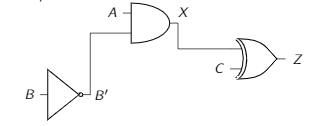
\includegraphics[frame]{logicgatediagram.png}} 
    
    \label{fig:graph}
   
\end{figure}
\column{0.5\textwidth}

\end{columns}
 \end{center}

\end{frame}

%\subsection{Literature}

\section{Solution}
\subsection{Propagation Delay}

\begin{frame}
\frametitle{Propagation Delay}
%\framesubtitle{Literature}

Propagation delay refers to the time taken by a signal to reach its destination.


%\item $\myvec{4 & 5}\vec{O} = 2 \ne 6 $. Incorrect.
%\vfill
%\item $\myvec{2 & -3}\vec{O} +10 = 0 $. Correct.
%\vfill
%\item $\myvec{3 & 4}\vec{O} = 2 \ne 3 $.  Incorrect.
%\vfill
%\item $\myvec{5 & 2}\vec{O} +4= -2 \ne 0 $. Incorrect
%\end{enumerate}
\end{frame}


\subsection{Timing Diagrams}
\begin{frame}{Solution / Timing Diagrams}
 \begin{center}
\begin{columns}
\column{1.15\textwidth}
\vspace{-0.45cm} % "\vspace" used to align picture vertically, preventing overflow
    \begin{figure}[h]
    \centering
   
        
    
    \scalebox{0.55} {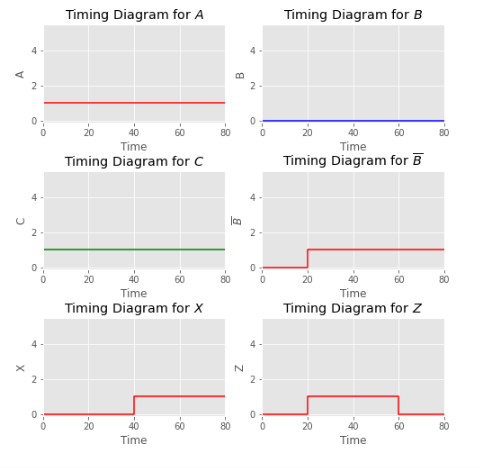
\includegraphics[frame]{timingdiagram.png}} 
    
    \label{fig:graph}
   
\end{figure}
\column{0.5\textwidth}

\end{columns}
 \end{center}
\end{frame}
    
%Let $\vec{O}$ be the centre of $C$. Then the equation of the normal, OQ is
%\begin{align}
%%\vec{x}^T\vec{x}-2\vec{O}^T\vec{x} +F = 0
%\myvec{0 & 1}\brak{\vec{O}-\vec{Q}} &= 0
%\nonumber \\ 
%\implies \myvec{0 & 1}\vec{O} = 2
%\label{eq:circle_7_o1}
%\end{align}
%%
%Also, 
%%Substituting \eqref{eq:circle_7_p} in \eqref{eq:circle_7_c}, 
%\begin{align}
%\norm{\vec{O}-\vec{P}}^2&=\norm{\vec{O}-\vec{Q}}^2 
%\nonumber \\
%\implies 2\brak{\vec{P}-\vec{Q}}^T\vec{O} &= \norm{\vec{P}}^2-\norm{\vec{Q}}^2 
%\nonumber \\
%\text{or, } \myvec{1 & -1}\vec{O} &= -4
%\label{eq:circle_7_o2}
%\end{align}
%%
%\eqref{eq:circle_7_o1} and \eqref{eq:circle_7_o2} result in the matrix equation
%\begin{align}
%\myvec{1 & -1 \\ 0 & 1}\vec{O} = \myvec{-4\\2}
%\label{eq:circle_7_matrix}
%\end{align}
%yielding the augmented matrix
%\begin{align}
%\myvec{1 & -1 & -4\\ 0 & 1 & 2} \leftrightarrow \myvec{1 & 0 & -2\\ 0 & 1 & 2}\implies \vec{O} = \myvec{-2 \\2}
%\label{eq:circle_7_o}
%\end{align}
%%
\end{frame}

\subsection{Truth Table}
\begin{frame}{Solution / Truth Table}
\begin{center}
\begin{columns}
\column{1.15\textwidth}
\vspace{1cm} % "\vspace" used to align picture vertically, preventing overflow
    \begin{figure}[h]
    \centering
   
        
    
    \scalebox{0.95} {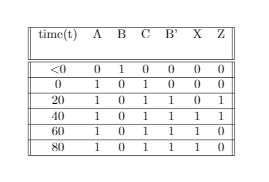
\includegraphics[frame]{truthtable.png}} 
    
    \label{fig:graph}
   
\end{figure}
\column{0.5\textwidth}

\end{columns}
 \end{center}
\end{frame}

%
%The radius  of $C$ is obtained as
%\begin{align}
%r = \norm{O-P} = 2
%\end{align}
\end{frame}
%\section{Plot}
\subsection{Conclusion}
\begin{frame}[fragile]
\frametitle{Conclusion}

According to the given timing diagram, Z=1 for a duration of 20-60ns.

\begin{center}
\begin{columns}
\column{1.15\textwidth}
\vspace{1cm} % "\vspace" used to align picture vertically, preventing overflow
    \begin{figure}[h]
    \centering
   
        
    
    \scalebox{0.55} {\includegraphics[frame]{timingdiagramZ.png}} 
    
    \label{fig:graph}
   
\end{figure}
\column{0.5\textwidth}

\end{columns}
 \end{center}
\end{frame}

%plots Fig. \ref{fig:circle_diameter}.
%
%\begin{figure}
%\centering
%\includegraphics[width=0.6\columnwidth]{./figs/circle_diameter.eps}
%\caption{Circle $C$ and all lines (i)-(iv). (ii) is a diameter.}
%\label{fig:circle_diameter}
%\end{figure}
\end{frame}
%\begin{frame}
%\frametitle{Introduction}
%\framesubtitle{Literature}
%%\begin{figure}[t!]
%%    \centering
%%    \begin{subfigure}[t]{0.4\columnwidth}
%%        \centering
%%        \includegraphics[width=\columnwidth]{point_source}
%%        \caption{Single point source}
%%\label{fig3:subfig1}        
%%    \end{subfigure}%
%%    ~ 
%%    \begin{subfigure}[t]{0.4\columnwidth}
%%        \centering
%%        \includegraphics[width=\columnwidth]{pointNoPowerDist_new}
%%        \caption{SNR profile}
%%\label{fig3:subfig2}
%%    \end{subfigure}
%%  %  \caption{Average SNR for a BPP. $N=16$}
%%    \label{fig3}
%%  \end{figure}
%
%\end{frame}
%  
%
%
%%



\end{document}
